\chapter{Equivalence of SGD and Frugal-1U}
\label{ch: algo_equal}

\graphicspath{{Figures/Frugal_SGD/}{./}} 

% --------------------------------------------------------------------------------
%                                Quantile Estimation
% --------------------------------------------------------------------------------
           
In 1978, the \textit{pinball loss} function was proposed by \citeauthor{koenkerRegressionQuantiles1978}\cite{koenkerRegressionQuantiles1978}, which is well-known for quantile estimation in both statistics and machine learning. In this chapter, we present the implementation of SGD approach with pinball loss on quantile estimation. We also illustrate that, in some degree, there is an equivalence relationship between our algorithm and the state-of-the-art Frugal-1U\cite{maFrugalStreamingEstimating2014} by both theoretical analysis and experimental results. After the introduction of pinball loss in section\ref{sec: pinball_loss}, section \ref{sec: derive_sgd} introduces the SGD methods and at the same time shows the equivalence to Frugal-1U by algorithm rephrasing. In addition, we offer some complementary explanation, supporting experiment results and further discussion for the proof of algorithm equivalence in section \ref{sec: algo_equivalence}.

\section{Pinball Loss for Quantile Estimation}
\label{sec: pinball_loss}
The pinball function is a convex loss function for estimation on a quantile value.
For a one-dimensional dataset $X = \{x_1, x_2, \cdots, x_N\}$, 
now consider the loss function for a single data point $x$ $(i \in {1, \cdots, N})$ on the $\tau$-quantile ($\tau \in (0,1)$).
Let $t := x - q$ be the difference between the real value $x$ and the estimate of quantile $q$.
The pinball loss function $l_{\tau}(\cdot): \R \to \R_{\geq 0}$ on $t$ is defined by

\begin{equation}
    l_\tau(t)= 
        \begin{cases}
            \tau t & t > 0\\
            -(1-\tau) t & otherwise
        \end{cases}
\end{equation}


And the $\tau$-quantile loss has the {\color{red} subgradient}:
\marginpar{Not sure to use subgradient or gradient and not mention $0$}

\begin{equation}
    \frac {\partial l_\tau(t)}{\partial t}= 
        \begin{cases}
            \tau                & t > 0\\
            -(1-\tau)           & t < 0\\
            [\tau, -(1 - \tau)] & t = 0
        \end{cases}
\end{equation}



The overall loss for distribution $X$ with quantile estimation $q$ is

\begin{equation}
    L_{\tau}(q) = \sum_{x \in X} l_{\tau}(x - q)
\end{equation}


The best estimate of the $\tau$-quantile $q$ is the $q$ with minimal overall loss. 
Let $q^\ast$ be the best estimate, then we have
\begin{equation}
    q^\ast = \argmin_{q} L_{\tau}(q)
\end{equation}



% --------------------------------------------------------------------------------
%                                SGD for Quantile Estimation
% --------------------------------------------------------------------------------
\section{Deriving the SGD approach from Frugal}
\label{sec: derive_sgd}
Inspired by Frugal-1U\cite{maFrugalStreamingEstimating2014}, we propose a quantile estimation method using the SGD approach with implementation of the pinball loss. Here this algorithm is introduced by the transformation of the Frugal-1U, which also provides an intuitive presentation of the algorithm equivalence. 

\subsection{Pseudo Code for the Frugal-1U Algorithm}

As a quantile estimation algorithm using constant memory storage, Frugal-1U reaches the extreme of memory usage for it "uses only one unit of memory per group to compute a quantile for each group"\cite{maFrugalStreamingEstimating2014}. Besides the minimal memory usage, the update methods is also computationally simple. Here is the pseudo code of Frugal-1U
\marginpar{the pseudo code has already been mentioned in literature review}
\begin{algorithm}
\caption{Frugal-1U}\label{alg:frugal_1U}
    \begin{algorithmic}[1]
        \Require{Data Stream $S$, $h$, $k$, $1$ unit of memory $\tilde{m}$}
        \Ensure{$\tilde{m}$}
        % \Procedure{frugal}{$X,\tau$}            \Comment{X is the dataset}
        \State {Initialization $\tilde{m} = 0$}               %\Comment{Default initialization $q_0$ = 0}
            \For{\textbf{each} $s_i$ in $S$}                  %\Comment{Parameter update for each input data point}
                \State{$rand$ = random(0,1)}
                \Comment{get a random value in $[0,1]$}
                % \State {\textbf{set} $\alpha_k$} \Comment{Set step size}
                \If{$s_i > \tilde{m}$ \textbf{and} $rand > 1-\frac{h}{k}$} %\Comment{$q_{k+1} = q_k + \alpha_k \tau$ when $x_k - q_k > 0$}
                    \State{$\tilde{m} = \tilde{m} + 1$;}
                \Else { \textbf{if} $s_i < \tilde{m}$ \textbf{and} $rand > \frac{h}{k}$}  %\Comment{$q_{k+1} = q_k - \alpha_k (1-\tau)$ otherwise}
                    \State{$\tilde{m} = \tilde{m} - 1$;}
                \EndIf
            \State{\textbf{end if}}
            \EndFor
        \State{\textbf{end for}}
        % \State \textbf{return} $q$              \Comment{$q_k$ is the SGD result of quantile estimate}
        % \EndProcedure
    \end{algorithmic}
\end{algorithm}
The output $\tilde{m}$ is the estimate of the $h$th $k$-quantile for a given data stream $S$. 
By rephrasing of some steps of Frugal-1U, 
its equilalence to an SGD algorithm for quantile estimation will be shown in the follwing part.
\\\\
\textbf{Rephrasing of the Algorithm} \label{replacements}
\begin{enumerate}
    \item The constant $\frac{h}{k}$ is replaced by $\tau$, since the $\tau$-quantile is defined
     as the $h$th $k$-quantile point in chapter \ref{ch: background}.
    % \item The quantile estimate $\tilde{m}$ is replaced by $q$, as it stands for estimate of quantile.
    \item The generation of random number and it's comparison with $1-\frac{h}{k}$ or $\frac{h}{k}$
    in line 3 to 7 is replaced by the following algorithm.
    \begin{algorithm}
        \begin{algorithmic}[1]
            \setcounter{ALG@line}{2}
            \State{ }   \Comment{No need to generate a random number}
            \If{$s_i > \tilde{m}$} %\Comment{$q_{k+1} = q_k + \alpha_k \tau$ when $x_k - q_k > 0$}
                \State{$\tilde{m} = \tilde{m} + 1 \times (1-\frac{h}{k})$}     
                \Comment{$P((rand > 1-\frac{h}{k}) \mid rand \in \mathcal{U}(0,1)) = 1-\frac{h}{k}$;}
            \Else { \textbf{if} $s_i < \tilde{m}$}  %\Comment{$q_{k+1} = q_k - \alpha_k (1-\tau)$ otherwise}
                \State{$\tilde{m} = \tilde{m} - 1 \times \frac{h}{k}$}         
                \Comment{$P((rand > \frac{h}{k}) \mid rand \in \mathcal{U}(0,1)) = \frac{h}{k}$;}
            \EndIf 
        \end{algorithmic}
    \end{algorithm}

    % Here the probability $P((rand > p) \mid rand \in \mathcal{U}(0,1))$ is the simplification
    % for the generation of random number $rand$ and it's comparison to a constant $p$ $(0 < p < 1)$.
    
    To understand this replacement, let's consider the serie of the 3 steps: 
    (i) generate a random number $rand$, 
    (ii) compare it with a constant $p$, and
    (iii) take action if $rand > p$. 
    It can be interpreted as take the action with probability 
    $P((rand > p) \mid rand \in \mathcal{U}(0,1))$. 

    Mathmatically, the replacement works because the expected change of
    $\tilde{m}$ in both methods are the same. 
    For example when $s_i > \tilde{m}$, 
    the expected change of $\tilde{m}$ is
    $E_1[\nabla \tilde{m}] = E[\tilde{m} \times p]$ in the Frugal-1U with 
    random number generation,
    while 
    $E_2[\nabla \tilde{m}] = \tilde{m} \times p$ in the replacement method.
    Since $E_1[\nabla \tilde{m}] = E_2[\nabla \tilde{m}]$, the replacement is valid
    with regard to the expectation of the change in quantile estimate during each step.

\end{enumerate}


\subsection{SGD for Loss function}

Let $q_0$ be the initial guess of quantile estimate. 
By SGD, the estimate is updated each step with a data point from the distribution.
\begin{equation}
    q_{k+1} = q_k - \alpha_k g_k
\end{equation}

where $ \alpha_k $ is a suitable step size and 

\begin{equation}
    g_k = \partial L_{\tau}^{(k)}(q_k) \in \frac{\partial l_\tau(x_k - q_k)}{\partial q_k}
\end{equation}
{Notice here partial is taken because the gradient of a single variable function equals the partial of it.}
\\\\
Then we have
\begin{equation*}
    q_{k+1} = 
    \begin{cases}
        q_k + \alpha_k \tau               & x_k - q_k > 0\\
        q_k - \alpha_k (1-\tau)           & x_k - q_k \leq 0\\
        % [\tau, -(1 - \tau)] & t = 0
    \end{cases}
\end{equation*}

\marginpar{
{\color{red} \textbf{Problem}}
In Frugal-1U the quantile estimate $q$ does not change when $x_k = q$, but in SGD 
the quantile estimate is updated: $q = q-\alpha_k (1-\tau)$. This can be seen as different
} 
\begin{algorithm}
    \caption{SGD algorithm}\label{alg:SGD}
    \begin{algorithmic}[1]
        \Require{Data Stream $X$, $\tau$, $1$ unit of memory $q$}
        \Ensure{$q$}
        % \Procedure{frugal}{$X,\tau$}            \Comment{X is the dataset}
        \State {Initialize} $q$                 \Comment{Default initialization $q_0$ = 0}
            \For{$x_k$ in $X$}                  \Comment{Parameter update for each input data point}
                \State \textbf{set} $\alpha_k = 1$  \Comment{Set step size}
                \If{$x_k > q$}                  \Comment{$q_{k+1} = q_k + \alpha_k \tau$ when $x_k - q_k > 0$}
                    \State{$q = q + \alpha_k \tau$}
                \Else                           \Comment{$q_{k+1} = q_k - \alpha_k (1-\tau)$ otherwise}
                    \State{$q = q - \alpha_k (1-\tau)$}
                \EndIf
            \EndFor
        \State \textbf{return} $q$              \Comment{$q_k$ is the SGD result of quantile estimate}
        % \EndProcedure
    \end{algorithmic}
\end{algorithm}
Besides the replacements mentioned in section \ref{replacements}, the notations have changed from Frugal-1U to SGD: 
$X$ is applied for the data stream, and $q$ instead of $\tilde{m}$ to represent quantile estimate. The other important potential change is the introduction of step size. Specifically, the step size is not mentioned in Frugal-1U because it is fixed as constant $1$. While the highlight of SGD algorithm is the choice of constant or variable step size $\alpha_k$ for each data point $x_k$. The flexibility of step size can be contributing for a better convergence rate when appropriate step sizes are chosen.


\textbf{subgradient} values for $l_\tau(x_k - q_k)$ 
{\color{red} \textbf{but then I need to explain subgradient descent}} 
% --------------------------------------------------------------------------------
%                              Equality of two algorithms 
% --------------------------------------------------------------------------------
\section{Equivalence of Algorithms}
\label{sec: algo_equivalence}

The derivation of the SGD algorithm from Frugal-1U has roughly shown the evident similarity between them. In this section, we investigate the similarity between our approach, that we refer to as SGD algorithm, and Frugal-1U, which leads to the proof of equivalence by experimental performances with additional discussion.

\subsection{Comparison experiments between SGD and Frugal-1U}

We investigate various aspects of the similarity between the SGD algorithm and the Frugal-1U algorithm: behaviours and results of different data distributions. The behavioural similarity is inspired by the \textit{behavioural equivalence} \cite{gurevichSequentialAbstractstateMachines2000}, which requires sequential algorithms to have same states, same initial states, and the same transition function for abstract state machine (ASM). The quantile estimation results are compared base on the final output results of the algorithms.

\subsubsection{Data distributions and algorithm settins}

For comprehensiveness, we evaluate the algorithms using data generated from three distributions:
    \begin{enumerate}
        \item a gaussian distribution with mean 2 and standard derivation 18 (\textit{gau-1})
        \item a mixed gaussian distribution composed of 5 gaussian distributions (\textit{mix}):
            \begin{enumerate}
                \item weight = 0.3, mean = 2, standard derivation = 7
                \item weight = 0.2, mean = 0, standard derivation = 0.7
                \item weight = 0.1, mean = 36, standard derivation = 26
                \item weight = 0.15, mean = 5, standard derivation = 77
                \item weight = 0.25, mean = -77, standard derivation = 7
            \end{enumerate}
            \item a exponential distribution with \textit{np.random.exponential(scale=1, size=datasize)*6.5 - 20} (\textit{mix})
            \marginpar{How to discribe the exponential distro?}
    \end{enumerate}
Each data stream contains 1000 randomly ordered samples from the corresponding distribution with a fixed sequence. The algorithms initialization both set their starting point of quantile estimate to $0$ for any quantile values. The step size of the SGD algorithm is set as constant 1.

\subsubsection{Evaluation methods}

For each simulation setup, we run the Frugal1U 100 times and SGD once. Since the data stream is fixed on both data points and sequence, the behaviour and result of SGD are also fixed, while Frugal1U is likely to perform differently given its randomness in each update steps. For a quantile probability $\tau$, let $\tau$-$q_{\text{batch}}$ be the computation results of the batch quantile, $\tau$-$q_{\text{SGD}}$ and $\tau$-$q_{\text{Frugal}}$ be the results respectively of SGD and Frugal1U algorithm. The similarity of the two estimates $S_\tau$ is measured by
\begin{equation}
    S_\tau = \frac{ \tau\text{-}q_{\text{SGD}} - \tau\text{-}q_{\text{Frugal}} }{ \tau\text{-}q_{\text{SGD}} - \tau\text{-}q_{\text{batch}} }
\end{equation}

And the behavioural similarity is measured by comparing the mean value of each Frugal step with each SGD step.


\subsubsection{Results for similarity comparisons}

\marginpar{I think more data is required, for example the mean and variance comparison on processes?}
\begin{figure}[h!]
    \centering
	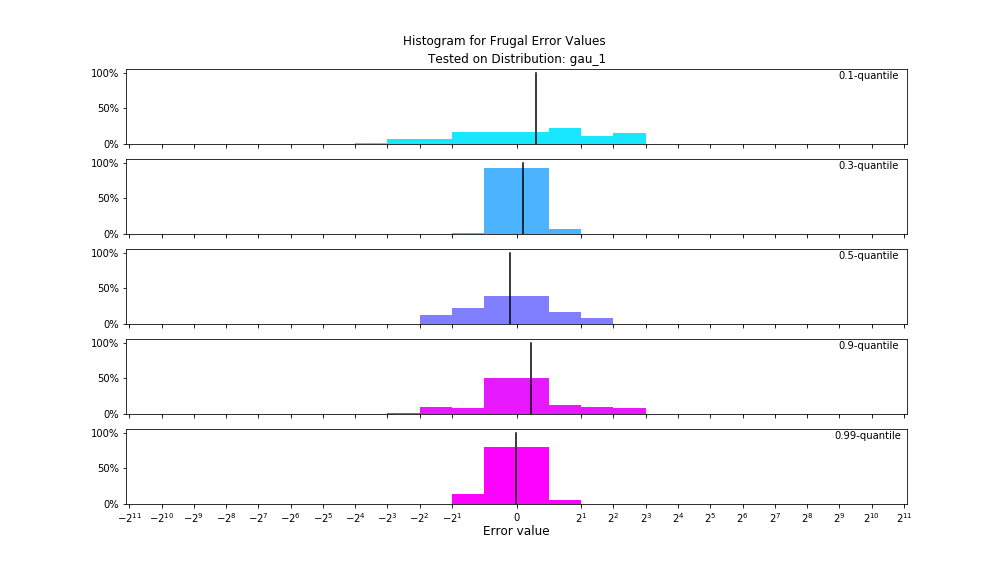
\includegraphics[width=1\columnwidth]{gau_1_err.png}
    \caption{Quantile estimation similarity comparison on dataset from gau-1}
    \label{fig: gau_1_err}
\end{figure}

\begin{figure}[h!]
    \centering
	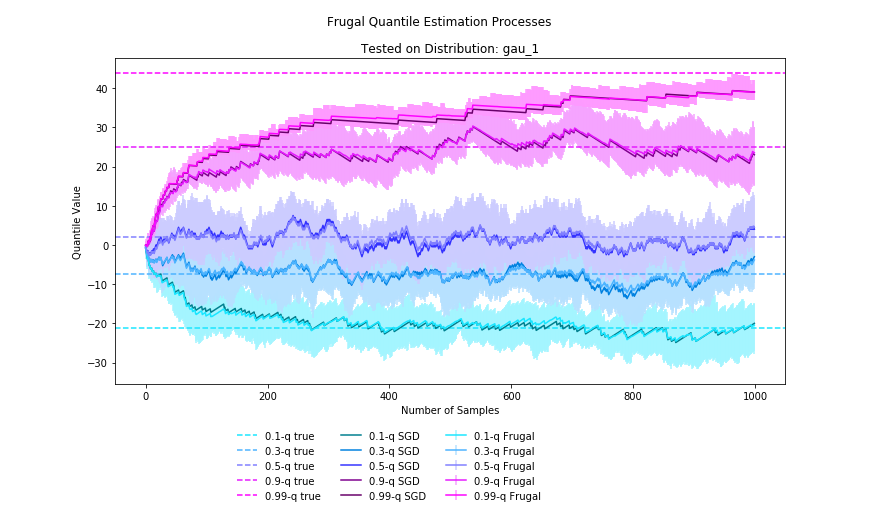
\includegraphics[width=1\columnwidth]{gau_1_proc.png}
    \caption{Quantile estimation similarity comparison on dataset from gau-1}
    \label{fig: gau_1_proc}
\end{figure}

\begin{figure}[h!]
    \centering
	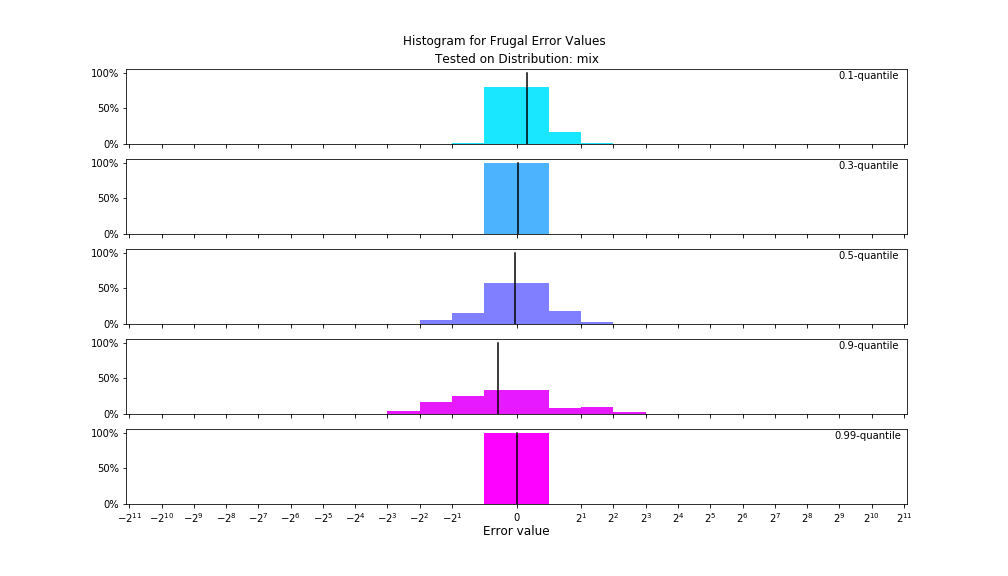
\includegraphics[width=1\columnwidth]{mix_err.png}
    \caption{Quantile estimation similarity comparison on dataset from mix}
    \label{fig: mix_err}
\end{figure}

\begin{figure}[h!]
    \centering
	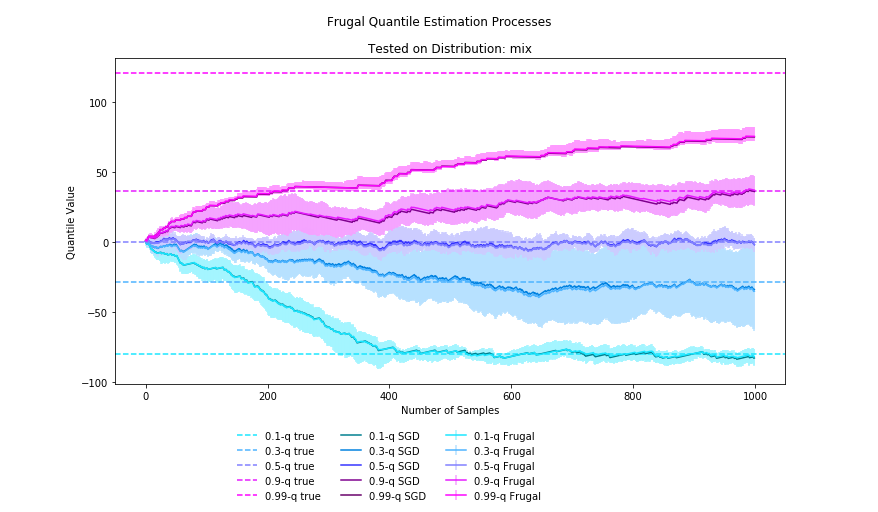
\includegraphics[width=1\columnwidth]{mix_proc.png}
    \caption{Quantile estimation similarity comparison on dataset from mix}
    \label{fig: mix_proc}
\end{figure}

\begin{figure}[h!]
    \centering
	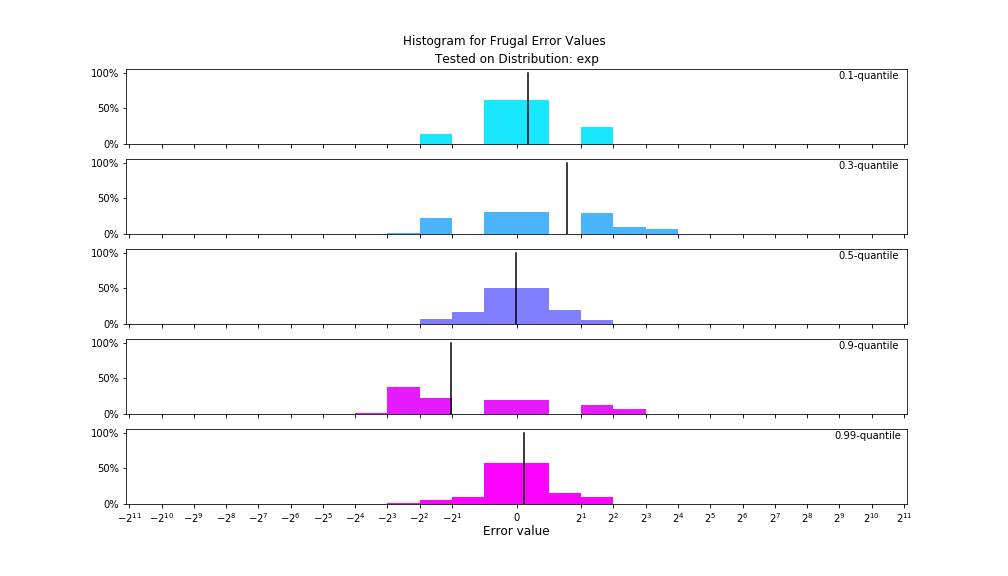
\includegraphics[width=1\columnwidth]{exp_err.png}
    \caption{Quantile estimation similarity comparison on dataset from exp}
    \label{fig: exp_err}
\end{figure}

\begin{figure}[h!]
    \centering
	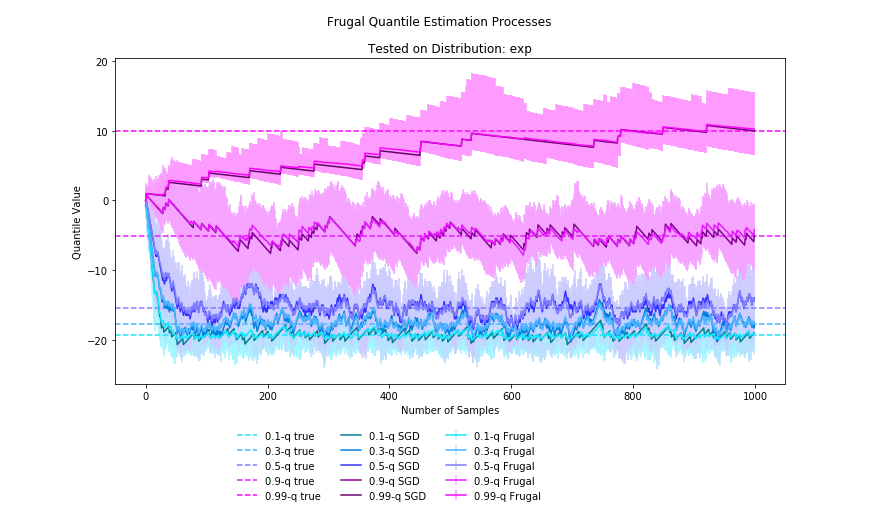
\includegraphics[width=1\columnwidth]{exp_proc.png}
    \caption{Quantile estimation similarity comparison on dataset from exp}
    \label{fig: exp_proc}
\end{figure}

\subsection{Discussion about the equivalence}
Although it is claimed in this paper that the SGD algorithm and the Frugal-1U is equivalent to some extent, \citeauthor{blassWhenAreTwo2008}\cite{blassWhenAreTwo2008} have already pointed that there is no such relation as equivalence between any two algorithms. 




